\documentclass{beamer}
\usepackage[utf8]{inputenc}
\usepackage{graphicx}
 \usetheme{CambridgeUS}
\title[Group Charlie --- Multi-Lingual SMS]{Group Charlie\\Multi-Lingual SMS}
\author[aw625, chw43, did23, sd660, tsp31]{Andrew, Chihang, Daria, Swaraj and Tanvi}
\institute[]{University of Cambridge}
\date{March 4, 2015}
\begin{document}
\maketitle

\begin{frame}
\frametitle{Background}
\setbeamertemplate{itemize items}[triangle]
\begin{itemize}[<+->]
\item Africa's Voices: Opinion polling done by broadcasting a variety of questions from several radio stations, where answers were received as SMS messages.
\item Main problem: The SMS messages were in different languages and sometimes included irrelevant information, such as details of the sender.
\item Sub-problem: Machine translation is not feasible for minority languages with little economic value. As a result of this, translation was taken to be an expensive task.
\item Problem we're trying to solve: allow for easy detection of opinion trends in such data, despite it being in several languages.
\end{itemize}
\end{frame}

\begin{frame}
\frametitle{Our goals}
\setbeamertemplate{itemize items}[triangle]
\begin{itemize}[<+->]
\item To create a visual browser that will allow international policy teams to observe trends.
\item This is a tool for scientists --- it should have a friendly and interactive UI while not getting in the way.
\item Due to translation being expensive, we need to allow for the researchers to determine more important words/topics for which they can prioritise translation.
\end{itemize}

\onslide<+->{Additional requirements set along the way:}

% \pause
\begin{itemize}[<+->]
\item Allow for identification of the language that a message was written in.
\item Allow for `cleaning up' of the data by removing names, {\tt txt-speak} and other slang.
\end{itemize}
\end{frame}

\begin{frame}
\setbeamertemplate{itemize items}[triangle]
\frametitle{Overview of the project}
The project has been implemented as a web application.\\
\pause
User input:
\pause
\begin{itemize}[<+->]
\item CSV file containing relevant columns (country, radio station, message)
\item Categories and respective keywords associated with them\\
Format --- {\tt {\bf Cat1}:\ KeyA, KeyB; {\bf Cat2}:\ KeyC, KeyD, KeyE}
\end{itemize}
\onslide<+->{Viewing `modes' implemented:}
\begin{itemize}[<+->]
\item Word cloud
\item Pie chart
\item Bar graph
\item Table view
\end{itemize}
\onslide<+->{A data manipulation page has also been added.}
\end{frame}

\begin{frame}
\frametitle{Word Cloud}
  \begin{figure}
    \centering
    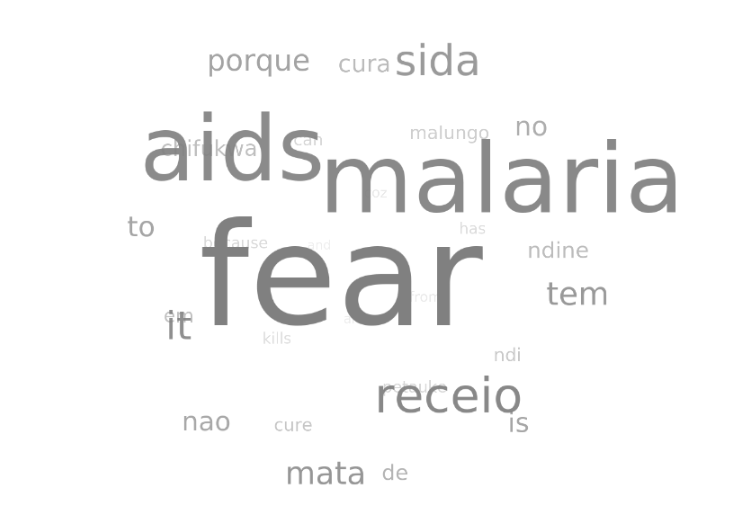
\includegraphics[scale=0.3]{./word.png}
    \caption{Word cloud --- useful for viewing major keywords/concerns}
  \end{figure}
\end{frame}

\begin{frame}
\frametitle{Pie Chart}
  \begin{figure}
    \centering
    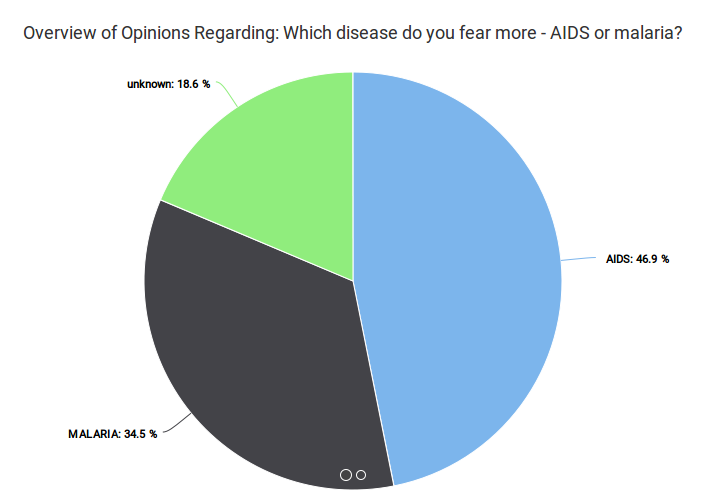
\includegraphics[scale=0.3]{./pie.png}
    \caption{Pie chart --- useful for viewing major opinions}
  \end{figure}
\end{frame}

\begin{frame}
\frametitle{Bar Graph}
  \begin{figure}
    \centering
    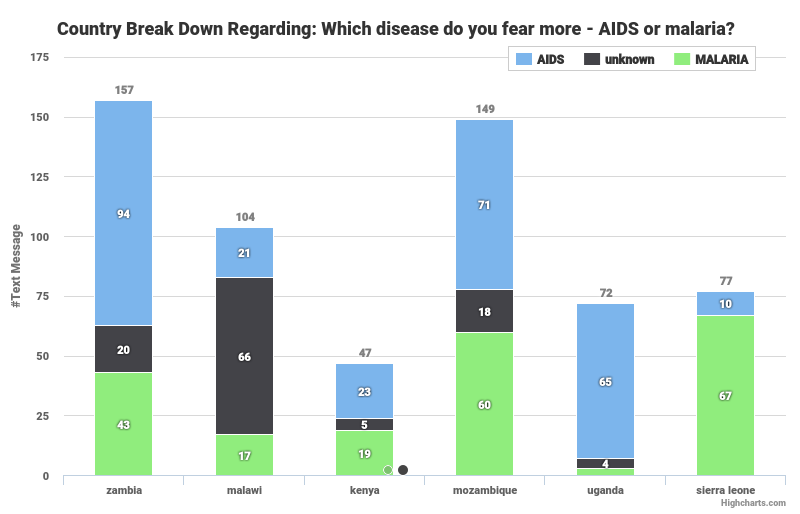
\includegraphics[scale=0.3]{./bar.png}
    \caption{Bar graph --- allows for breakdown by country}
  \end{figure}
\end{frame}

\begin{frame}
\frametitle{Table View}
  \begin{figure}
    \centering
    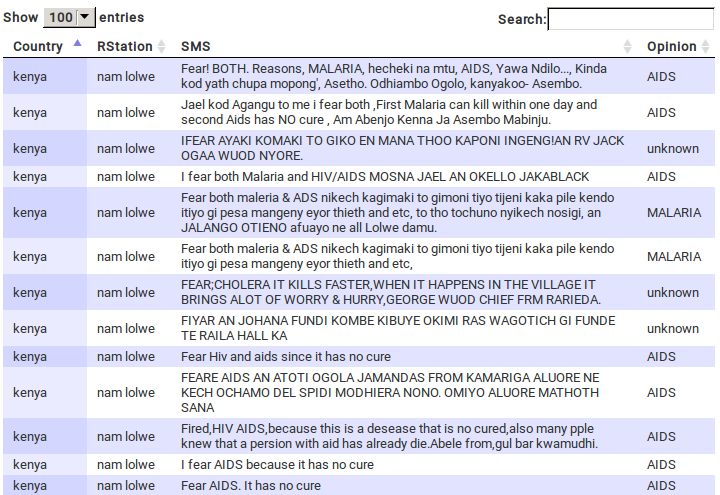
\includegraphics[scale=0.3]{./table.png}
    \caption{Table view --- used to view individual SMS messages}
  \end{figure}
\end{frame}

\begin{frame}
\frametitle{Data Manipulation}
  \begin{figure}
    \centering
    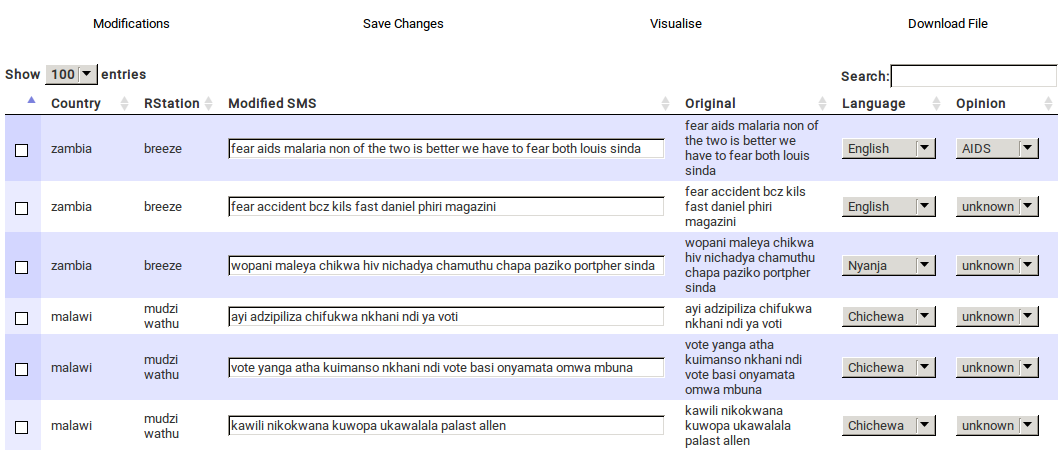
\includegraphics[scale=0.3]{./manip.png}
    \caption{Data manipulation --- used to modify/correct data}
  \end{figure}
\end{frame}

% Talk about general workflow at some point

\begin{frame}
\frametitle{Technical details}
\end{frame}

\begin{frame}
\frametitle{Lessons learned}
\setbeamertemplate{itemize items}[triangle]
\begin{itemize}[<+->]
\item I hate SWEng
\end{itemize}
\end{frame}

\begin{frame}[c]
\begin{center}
\Huge Thanks for listening!
\end{center}
\end{frame}

\end{document}
